% !TEX root = ../notes_unsupervisedlearning.tex
% Chapter 9: Self-Supervised Learning
%%%%%%%%%%%%%%%%%%%%%%%%%%%%%%%%%%%%%%%%%%%%%%%%%%%%%%%%%%%%%%%%%%%%%%

\chapter{Self-Supervised Learning}\index{Self-Supervised Learning}\index{contrastive learning}\index{SimCLR}\index{BERT}\index{CLIP}
\newthought{Letting data supervise itself.}

% ==============================================================================================
% BLOCK 1: INTRODUCTION
% ==============================================================================================

\section{The Why}\index{self-supervised learning}\index{pretext task}

\marginnote{\newthought{ImageNet} absorbed years of human effort to assemble fourteen million labelled images. The open web holds a hundred billion images that no curator will ever touch. The asymmetry between labelled and unlabelled data is the structural fact that motivates this chapter.}

\newthought{In the previous chapter} we learned that a model's reliability is bounded by the distribution it was trained on.
Uncertainty estimation could tell us when an input falls outside that distribution; it could not extend the distribution itself.
Extending the distribution means more data, and the bottleneck is almost always the same: somebody had to annotate every training example by hand.

\newthought{Labels are scarce and expensive while unlabelled data is abundant.}
The internet, sensor networks, scientific instruments, and surveillance cameras all produce orders of magnitude more raw data than any annotation budget can keep up with.
The natural question is whether the structure of unlabelled data, on its own, carries enough signal to teach a model what to look at.

\newthought{Annotation cost} is the first wall.
ImageNet absorbed years of human effort to assemble fourteen million labelled images.
Medical imaging annotations cost between fifty and five hundred dollars per expert label, and each label requires a clinician.
An hour of autonomous driving footage takes longer to label, frame by frame and bounding box by bounding box, than it took to record.
Scaling labelled data linearly with model size is not a research challenge; it is a procurement problem with no obvious solution.

\newthought{Annotation bias} is the second wall.
Humans encode their priors when they label.
A clinician trained at one hospital draws boundaries that a clinician trained elsewhere would draw differently; a crowd-sourced labeller follows the instructions and the examples in front of them, not the underlying concept.
Curated datasets carry curator-specific structure that the model then inherits as a hidden assumption about the world.

\newthought{Scalability ceiling} is the third wall.
As model and data scale up, the bottleneck is no longer compute or storage; it is the human in the labelling loop.
A model that can train on ten times more data than today is useless if the labelling pipeline cannot grow with it, and the labelling pipeline cannot grow without an army of humans.

\newthought{Domain transfer cost} is the fourth wall.
Every new domain demands new labels.
A classifier trained on natural images cannot be deployed in a satellite-imagery pipeline without a new round of annotation; a medical model trained on adult patients needs paediatric labels before it can serve paediatric care.
Removing the human from the labelling loop opens the door to domain transfer that does not require starting over.

\newthought{Self-supervised learning closes this gap by extracting supervision from the data itself.}
Instead of asking a human what an image contains, we design a pretext task whose label can be read off directly from the data structure.
Rotate the image and ask the network to predict the rotation; mask out a patch and ask it to fill the patch in; take two random crops of the same image and ask whether they came from the same source.
None of these signals require annotation, yet each one becomes solvable only if the network has internalised something about object shape, texture, or semantics along the way.
The representations learned to solve the pretext task are the real product; the task itself is just scaffolding that the representations climb during training.

\newthought{In order to move from expensive manual annotation to learning from raw data} we have good reason to find ways to,
\begin{itemize}
    \item design auxiliary tasks whose supervision signal is inherent in the data itself, so that scale is bounded by storage rather than by human effort.
    \item learn representations that capture semantic structure without any human labels, transferable across downstream tasks the model was never explicitly trained for.
    \item understand what prevents collapse when the loss has no negatives to push against, and what makes one pretext task transfer better than another.
\end{itemize}

\newthought{The fundamental question} this chapter answers is whether the structure of unlabelled data carries enough signal to teach a model what to look at, without any human ever telling it what to value.

\subsection{Hands On Experience}

\newthought{Consider} the canonical six points unlabelled.
There is no class label, no ground truth, no oracle to tell the model which points belong together.

\begin{figure}
\centering
\begin{tikzpicture}
    \begin{axis}[
        xmin=0, xmax=10,
        ymin=0, ymax=10,
        width=0.5\textwidth, height=0.5\textwidth,
        axis line style={draw=none},
        tick style={black, thick},
        xtick={1,2,3,6,8}, ytick={1,2,3,7,8,9},
        xticklabel style={font=\small},
        yticklabel style={font=\small},
        tick align=outside, tick pos=left,
    ]
    \addplot[only marks, mark=*, mark size=2pt, black] coordinates {
        (1,2) (2,3) (3,1)
    };
    \addplot[only marks, mark=*, mark size=2pt, black!55] coordinates {
        (6,8) (8,7) (8,9)
    };
    \end{axis}
\end{tikzpicture}
\caption{Six unlabelled data points, the canonical example from the rest of the course. Can you design a pretext task that teaches a model which points belong together, without any labels?}
\label{fig:ssl_handson}
\end{figure}

\marginnote{\newthought{Three open questions.} How would you teach a model that some pairs of points are similar, without telling it which pairs? What transformation of these data points would yield a free supervision signal? What property of the data structure makes that supervision come for free?}

\newthought{The geometry already carries a signal} that a clever pretext task can convert into supervision.
If you take any one of the six points and apply a small perturbation, you get a new point that is almost the same; if you take a different point, the new point is far away.
The model never needs to know which point is which; it only needs to know that two perturbations of the same point should be close in feature space, while perturbations of different points should be far apart.

\newthought{A supervised classifier sits idle here.}
With no labels, gradient descent has nothing to push against.
Cross-entropy needs a target; mean squared error needs a target; the standard supervised pipeline halts at the first batch.
The data is rich, the labels are absent, and the supervised toolbox has no entry point.

\newthought{Self-supervised learning fabricates a target from the data itself.}
Two crops of the same image, two adjacent words in the same sentence, the rotation angle of an artificially rotated image, all of these are signals the data provides for free.
The model trains on whatever target the pretext task constructs, and the representations it learns along the way are usable for the real task we care about.

\begin{marginfigure}
\centering
\begin{tikzpicture}
    \begin{axis}[
        xmin=0, xmax=10,
        ymin=0, ymax=10,
        width=\marginparwidth, height=\marginparwidth,
        axis line style={draw=none},
        tick style={black, thin},
        xtick={1,3,5,7,9}, ytick={1,3,5,7,9},
        xticklabel style={font=\tiny},
        yticklabel style={font=\tiny},
        tick align=outside, tick pos=left,
    ]
    \addplot[only marks, mark=*, mark size=2pt, black] coordinates {(1,2)};
    \addplot[only marks, mark=*, mark size=2pt, black!30] coordinates {(1.3,2.4) (0.8,1.7)};
    \addplot[only marks, mark=*, mark size=2pt, black!55] coordinates {(8,7)};
    \draw[<->, thin, black] (axis cs:1.3,2.4) -- (axis cs:0.8,1.7);
    \draw[<->, densely dashed, thin, black!55] (axis cs:0.8,1.7) -- (axis cs:8,7);
    \end{axis}
\end{tikzpicture}
\caption{Two perturbations of $x_1$ (light grey) form a positive pair pulled together (solid). A perturbation of a different point $x_5$ is a negative pushed apart (dashed). The data, not the human, supplies the supervision.}
\label{fig:ssl_handson_pull_push}
\end{marginfigure}

\vspace{2.5em}

\newthought{The Learning Objectives} of this lecture:
\begin{itemize}
    \item Design pretext tasks and contrastive objectives that yield transferable representations from unlabelled data.
    \item Distinguish contrastive methods from non-contrastive and masked-prediction approaches, and identify what prevents representation collapse in each.
    \item Apply masked prediction across modalities and explain why cross-modal pre-training enables zero-shot transfer.
\end{itemize}


% ==============================================================================================
% BLOCK 2: MAIN THEORY
% ==============================================================================================

\newpage

\subsection{Pretext Tasks}\index{pretext task}

\marginnote{\newthought{A pretext task} creates pseudo-labels from data structure. The label is a function of the input itself, so no human is needed in the loop.}

\newthought{Early self-supervised methods} for vision designed clever pretext tasks by hand.
Each task takes an unlabelled image, applies a deterministic transformation, and asks the network to undo or identify the transformation.
The transformation parameters serve as the label, free of charge.

\newthought{The recipe is universal across tasks.}
Take an unlabelled input.
Apply a deterministic transformation parameterised by a known value.
Train the network to recover that value from the transformed input.
The recovered value is the supervision; the network learns whatever representation is required to solve the task.

\begin{table*}[ht]
\centering
\begin{tabular}{p{0.22\textwidth}p{0.40\textwidth}}
    \toprule
    \textbf{Task} & \textbf{Supervision Signal} \\
    \midrule
    Rotation prediction & Predict the rotation angle from $\{0, 90, 180, 270\}$ degrees \\
    Jigsaw puzzle       & Predict the permutation that shuffled image patches \\
    Colorization        & Predict the original colours from a grayscale input \\
    Inpainting          & Predict the pixel content of a missing region \\
    Context prediction  & Predict the relative position of two image patches \\
    \bottomrule
\end{tabular}
\vspace{2em}
\caption{Classic pretext tasks for images. Each task derives its supervision signal from the structure of the data itself, so the model can train on any image collection without a single human annotation.}
\label{tab:pretext_tasks}
\end{table*}

\newthought{Notice that the label is always derivable from the input.}
There is no separate annotation step, no expert in the loop, no curated labelling protocol.
Any unlabelled image can become a training example for any of these tasks just by applying the transformation in software.

\newthought{The limitation of handcrafted pretext tasks} is that solving them well does not always produce features that transfer well to downstream tasks.
A network can become very good at predicting rotation by latching onto a few low-level cues, watermark orientation or sky-on-top priors, that are useless for downstream classification.
The pretext task did its job; the representations it produced did not generalise.

\newthought{Handcrafted invariances do not transfer.}
What we need is a more principled pretext signal, one that forces the network to capture the kind of structure that any downstream task will benefit from, not just the structure required to solve one fixed task.


\subsection{Contrastive Learning}\index{contrastive learning}\index{InfoNCE}

\marginnote{\newthought{Core idea:} pull similar things together, push different things apart. Similarity is defined by the data, not by a human label.}

\newthought{Contrastive learning} reframes the pretext task around a single relational principle.
Take two augmented views of the same image and call them a positive pair; take views of different images and call them negatives.
Train the encoder so positive pairs land close together in feature space and negatives land far apart.
The supervision signal is now relational: the data tells the model which pairs should be similar simply by virtue of having come from the same source.

\newthought{The pretext task is no longer a guess about what features matter.}
We do not have to design rotation prediction or jigsaw and hope the resulting features generalise.
We only have to choose augmentations that preserve semantic content, and the contrastive loss does the rest.
The space of augmentations becomes the space of inductive biases the model inherits.

\newthought{The InfoNCE loss}\cite{vanDenOord2018InfoNCE} formalises this principle as a contrastive prediction problem.
Given an anchor representation $z$, a positive $z^+$, and a set of negatives $\{z^-_k\}$, the loss is the cross-entropy of identifying the positive among all candidates:

\begin{align}
    \mathcal{L}_{\text{InfoNCE}} &= -\log \frac{\exp(\text{sim}(z, z^+) / \tau)}{\exp(\text{sim}(z, z^+) / \tau) + \sum_k \exp(\text{sim}(z, z^-_k) / \tau)}
    \label{eq:infonce}
\end{align}

where $\text{sim}(u, v) = u \cdot v / (\|u\|\,\|v\|)$ is cosine similarity and $\tau$ is a temperature controlling the sharpness of the distribution.

\newthought{Notice that the loss is just a softmax classification.}
The positive plays the role of the correct class; the negatives play the role of the wrong classes; the model learns to assign high similarity to the positive and low similarity to the negatives.
Negatives do not need to be hard; they need to be many.
Each additional negative adds one more candidate to the denominator and tightens the constraint that the positive must beat.

\newthought{The temperature $\tau$} controls how aggressively the softmax responds to similarity differences.
Low temperature pushes the softmax toward a hard maximum, so the loss focuses gradient on the hardest negatives, those with similarity nearly as high as the positive.
High temperature smooths the distribution and treats all negatives more uniformly, so even easy negatives contribute to the gradient.
The optimal $\tau$ depends on how informative the negatives are; in practice, $\tau \approx 0.1$ has been found to balance focus on hard negatives against numerical stability.

\begin{figure}
\centering
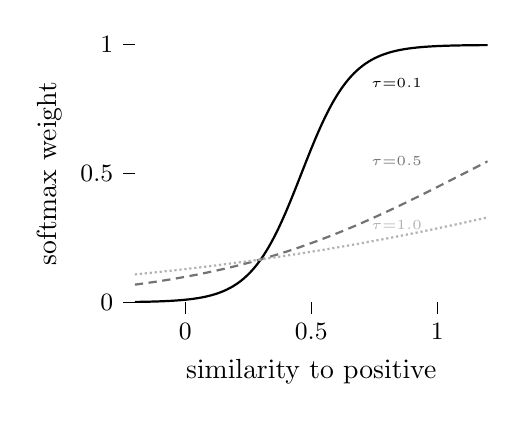
\begin{tikzpicture}
    \begin{axis}[
        xlabel={similarity to positive}, ylabel={softmax weight},
        xmin=-0.2, xmax=1.2, ymin=0, ymax=1,
        width=0.5\textwidth, height=0.4\textwidth,
        axis line style={draw=none},
        tick style={black, thin},
        xtick={0,0.5,1}, ytick={0,0.5,1},
        xticklabel style={font=\small},
        yticklabel style={font=\small},
        tick align=outside, tick pos=left,
        samples=120, domain=-0.2:1.2,
    ]
    \addplot[black, thick] {exp(x/0.1)/(exp(x/0.1)+5*exp(0.3/0.1))};
    \addplot[black!55, thick, densely dashed] {exp(x/0.5)/(exp(x/0.5)+5*exp(0.3/0.5))};
    \addplot[black!30, thick, densely dotted] {exp(x/1.0)/(exp(x/1.0)+5*exp(0.3/1.0))};
    \node[font=\tiny, anchor=west] at (axis cs:0.7,0.85) {$\tau{=}0.1$};
    \node[font=\tiny, black!55, anchor=west] at (axis cs:0.7,0.55) {$\tau{=}0.5$};
    \node[font=\tiny, black!30, anchor=west] at (axis cs:0.7,0.30) {$\tau{=}1.0$};
    \end{axis}
\end{tikzpicture}
\caption{The same input similarities produce different softmax weights at different temperatures. Low $\tau$ saturates the softmax: the positive's weight is near 1, the negatives near 0, and gradient flows almost entirely from the closest competitor. High $\tau$ flattens the distribution: every negative contributes, but the gradient on the positive shrinks.}
\label{fig:infonce_temperature}
\end{figure}

\begin{figure}
\centering
\begin{tikzpicture}[
    every node/.style={font=\small, align=center},
    block/.style={rectangle, draw=black, thick, rounded corners=2pt,
                  minimum width=1.6cm, minimum height=0.7cm, inner sep=4pt},
    arr/.style={-{Triangle[length=4pt, width=4pt, fill=black!70]}, thick, black!70},
]
    \node[block] (orig) at (0,0) {$x$};
    \node[block] (aug1) at (2.6, 1.0) {$x_1$};
    \node[block] (aug2) at (2.6,-1.0) {$x_2$};
    \node[block, fill=black!8] (enc1) at (5.0, 1.0) {$f$};
    \node[block, fill=black!8] (enc2) at (5.0,-1.0) {$f$};
    \node[block] (z1)   at (7.4, 1.0) {$z_1$};
    \node[block] (z2)   at (7.4,-1.0) {$z_2$};

    \draw[arr] (orig.east) -- node[above, font=\tiny, sloped] {aug} (aug1.west);
    \draw[arr] (orig.east) -- node[below, font=\tiny, sloped] {aug} (aug2.west);
    \draw[arr] (aug1) -- (enc1);
    \draw[arr] (aug2) -- (enc2);
    \draw[arr] (enc1) -- (z1);
    \draw[arr] (enc2) -- (z2);

    \draw[<->, thick, black] (z1.south) -- node[right, font=\tiny] {pull} (z2.north);

    \node[block, fill=black!2] (zneg) at (7.4,-3.0) {$z^-$};
    \draw[<->, thick, black!55, densely dashed] (z2.south) -- node[right, font=\tiny] {push} (zneg.north);
\end{tikzpicture}
\caption{Contrastive learning. Two augmented views $x_1, x_2$ of the same input $x$ pass through a shared encoder $f$ to produce representations $z_1, z_2$ that should be pulled together. Representations of different inputs $z^-$ should be pushed apart.}
\label{fig:contrastive_learning}
\end{figure}

\newthought{InfoNCE is silent on what the positive pair should look like.}
The choice of augmentation is everything; the same loss with weak augmentations produces collapsed representations, with strong augmentations produces useful ones.
The next subsection looks at the simplest concrete realisation, where the augmentation pipeline does almost all the work.


\subsection{SimCLR}\index{SimCLR}

\marginnote{\newthought{SimCLR.} Simple Contrastive Learning of Visual Representations\cite{Chen2020SimCLR}. The simplest realisation of the contrastive idea, and a strong baseline.}

\newthought{SimCLR} is the simplest realisation of the contrastive idea, and it works surprisingly well.
For each minibatch of $N$ images, generate two augmented views per image to obtain $2N$ samples.
For every positive pair $(i, j)$ taken from the same source image, treat the remaining $2(N-1)$ samples in the batch as negatives, and apply the InfoNCE loss.

\begin{algorithm}[H]
\caption{SimCLR}
\begin{algorithmic}[1]
\Require Minibatch of $N$ images, encoder $f$, projection head $g$, temperature $\tau$
\For{each minibatch of $N$ images}
    \State Generate $2N$ augmented views, two per image
    \For{each positive pair $(i, j)$}
        \State $z_i \gets g(f(x_i))$ \Comment{encoder $f$ then projection head $g$}
        \State $z_j \gets g(f(x_j))$
        \State Treat the other $2(N-1)$ views as negatives
        \State Compute InfoNCE loss using Equation~\ref{eq:infonce}
    \EndFor
\EndFor
\end{algorithmic}
\end{algorithm}

\newthought{Notice that the projection head $g$ exists only during training.}
After training, $g$ is discarded and the encoder $f$ alone is used as the feature extractor for downstream tasks.
The projection head absorbs the augmentation-specific transformations during training; the encoder, freed from this duty, learns a more general representation.

\begin{figure}
\centering
\begin{tikzpicture}[
    every node/.style={font=\small, align=center},
    block/.style={rectangle, draw=black, thick, rounded corners=2pt,
                  minimum width=1.6cm, minimum height=0.7cm, inner sep=4pt},
    arr/.style={-{Triangle[length=4pt, width=4pt, fill=black!70]}, thick, black!70},
]
    \node[block] (input) at (0,0) {$x$};
    \node[block] (aug1) at (2.4, 1.4) {$x_1$};
    \node[block] (aug2) at (2.4,-1.4) {$x_2$};
    \node[block, fill=black!8] (f1) at (4.6, 1.4) {$f$};
    \node[block, fill=black!8] (f2) at (4.6,-1.4) {$f$};
    \node[block, fill=black!2] (g1) at (6.8, 1.4) {$g$};
    \node[block, fill=black!2] (g2) at (6.8,-1.4) {$g$};
    \node[block] (z1) at (9.0, 1.4) {$z_1$};
    \node[block] (z2) at (9.0,-1.4) {$z_2$};
    \node[font=\small] (loss) at (10.8, 0) {$\mathcal{L}_{\text{InfoNCE}}$};

    \draw[arr] (input) -- node[above, font=\tiny, sloped] {augment} (aug1);
    \draw[arr] (input) -- node[below, font=\tiny, sloped] {augment} (aug2);
    \draw[arr] (aug1) -- (f1);
    \draw[arr] (aug2) -- (f2);
    \draw[arr] (f1) -- (g1);
    \draw[arr] (f2) -- (g2);
    \draw[arr] (g1) -- (z1);
    \draw[arr] (g2) -- (z2);
    \draw[arr] (z1.east) -- (loss.north west);
    \draw[arr] (z2.east) -- (loss.south west);
\end{tikzpicture}
\caption{SimCLR architecture. Two augmentations of the same input pass through a shared encoder $f$ and a shared projection head $g$ to give $z_1, z_2$, which are pulled together by InfoNCE while every other view in the batch contributes a negative pair. After training, $g$ is discarded; only $f$ ships.}
\label{fig:simclr_arch}
\end{figure}

\newthought{Four ingredients carry the method.}
The augmentation pipeline combines random crop, colour jitter, and Gaussian blur, and the strength of the augmentation determines what invariances the representation acquires; weak augmentations let the network rely on shortcut features.
A small projection head $g$, an MLP, sits between the encoder $f$ and the loss; it absorbs augmentation-specific transformations during training and is then discarded so that the downstream representation lives at the encoder output, where it is more general.
Large batch sizes, in the thousands, supply enough negatives to make the contrastive task informative; with too few negatives, the loss saturates and the gradient signal weakens.
A temperature around $\tau \approx 0.1$ has been found to balance focus on hard negatives against numerical stability.

\marginnote{\newthought{Practical protocol for SimCLR.} Augmentation set: random resized crop, colour jitter, Gaussian blur. Batch size: at least $1024$, often $4096$ or more. Projection head: two-layer MLP with hidden dim $2048$, output dim $128$. Temperature: $0.1$. Encoder: ResNet-50 or larger. Train: $200$+ epochs. Linear evaluation: train a linear classifier on top of the frozen encoder to measure feature quality.}

\newthought{The cost of SimCLR sits in the batch.}
Holding thousands of images in memory just to generate enough negatives is wasteful, and it puts contrastive learning out of reach for anyone without large accelerator clusters.
Momentum Contrast solves this with two design choices that decouple the negative pool from the batch size.


\subsection{MoCo: Momentum Contrast}\index{MoCo}\index{momentum encoder}

\marginnote{\newthought{MoCo.} Momentum Contrast\cite{He2020MoCo} decouples the negative pool from the batch size, so contrastive learning runs at modest batch sizes.}

\newthought{Momentum Contrast}\cite{He2020MoCo} solves the batch-size problem with two design choices.
A queue of recent embeddings serves as the negative pool, decoupling the number of negatives from the batch size.
A momentum encoder, a slowly updated copy of the online encoder, generates the keys that populate the queue, ensuring the keys remain consistent over time even as the online encoder evolves.

\newthought{The momentum update}\cite{He2020MoCo} for the key encoder weights is:

\begin{align}
    \theta_k &\gets m\, \theta_k + (1 - m)\, \theta_q
    \label{eq:moco_update}
\end{align}

with momentum $m = 0.999$, where $\theta_q$ are the online encoder weights and $\theta_k$ are the key encoder weights.

\newthought{The slow update is the point.}
A queue filled with embeddings from a rapidly changing encoder would be a queue of inconsistent keys, and the contrastive loss would chase a moving target.
With $m = 0.999$, the key encoder lags the online encoder by about a thousand updates; old queue entries remain comparable to fresh ones because the encoder that produced them has barely changed.

\begin{figure}
\centering
\begin{tikzpicture}[
    every node/.style={font=\small, align=center},
    block/.style={rectangle, draw=black, thick, rounded corners=2pt,
                  minimum width=1.6cm, minimum height=0.7cm, inner sep=4pt},
    arr/.style={-{Triangle[length=4pt, width=4pt, fill=black!70]}, thick, black!70},
    moarr/.style={-{Triangle[length=4pt, width=4pt, fill=black!30]}, thick, black!30, densely dashed},
]
    \node[block] (xq) at (0,1.5) {$x^q$};
    \node[block] (xk) at (0,-1.5) {$x^k$};
    \node[block, fill=black!8] (fq) at (2.6,1.5) {$f_q$};
    \node[block, fill=black!4] (fk) at (2.6,-1.5) {$f_k$};
    \node[block] (q) at (5.0,1.5) {$q$};
    \node[block] (k) at (5.0,-1.5) {$k$};
    \node[block, fill=black!2, minimum width=2.6cm] (queue) at (7.8,-1.5) {queue of $K$ keys};

    \draw[arr] (xq) -- (fq);
    \draw[arr] (xk) -- (fk);
    \draw[arr] (fq) -- (q);
    \draw[arr] (fk) -- (k);
    \draw[arr] (k) -- (queue);
    \draw[moarr] (fq.south) to[bend left=20] node[right, font=\tiny] {momentum} (fk.north);

    \node[font=\small] (loss) at (7.8,1.5) {$\mathcal{L}_{\text{InfoNCE}}$};
    \draw[arr] (q.east) -- (loss.west);
    \draw[arr] (queue.north) -- (loss.south);
\end{tikzpicture}
\caption{MoCo architecture. The query encoder $f_q$ trains via gradient descent. The key encoder $f_k$ is updated as a slow exponential moving average of $f_q$ (dashed). The queue stores the most recent $K$ keys, providing a large pool of consistent negatives without holding them in the current batch.}
\label{fig:moco_arch}
\end{figure}

\newthought{The result} is contrastive learning that trains effectively at batch sizes of $256$, several orders of magnitude smaller than SimCLR's optimal regime, with a queue of typically $K = 65{,}536$ negatives.
The same accuracy is reachable on commodity hardware that cannot fit a SimCLR batch.

\begin{table*}[ht]
\centering
\begin{tabular}{p{0.18\textwidth}p{0.16\textwidth}p{0.16\textwidth}p{0.20\textwidth}}
    \toprule
    \textbf{Property} & \textbf{SimCLR} & \textbf{MoCo} & \textbf{Notes} \\
    \midrule
    Negative pool       & $2(N-1)$ in-batch & queue of $K$         & MoCo decouples from batch \\
    Typical batch size  & $4096$            & $256$                & $16\times$ smaller \\
    Memory footprint    & batch-dominated   & queue + batch        & MoCo fits commodity GPUs \\
    Negatives per loss  & $\sim 8000$       & $\sim 65000$         & MoCo wins on negative count \\
    Encoder update      & gradient on $f$   & EMA on $f_k$         & MoCo introduces second encoder \\
    Hardware demand     & many GPUs         & one GPU sufficient   & Accessibility tilt \\
    \bottomrule
\end{tabular}
\vspace{2em}
\caption{SimCLR and MoCo compared. Both optimise InfoNCE on positive pairs and use augmentations as the positive-pair generator. The difference is engineering: SimCLR pays the cost in batch size, MoCo pays it in queue maintenance and a second encoder.}
\label{tab:simclr_vs_moco}
\end{table*}

\newthought{Contrastive losses need negatives.}
That, at least, was the conventional wisdom.
A line of work starting with BYOL showed that the constant-collapse solution can be avoided by structural choices alone, with no negative examples in the loss at all.


\subsection{Non-Contrastive Methods}\index{non-contrastive learning}\index{BYOL}\index{SimSiam}

\marginnote{\newthought{Surprising finding:} you do not need negatives at all. The loss can be entirely positive, and the network still avoids the constant solution.}

\newthought{Contrastive losses need negatives} to prevent the trivial solution of mapping every input to the same constant.
That, at least, was the conventional wisdom.
A line of work starting with BYOL showed the constant solution can be avoided by structural choices alone, with no negative examples in the loss.
This is the first major paradigm shift since contrastive learning itself: a working pretext task whose loss has only positive pairs.

\vspace{1.5em}

\newthought{BYOL: Bootstrap Your Own Latent.}\index{BYOL}\cite{Grill2020BYOL}
The online network has an encoder, a projector, and a small predictor head; the target network has only an encoder and a projector, and its weights are an exponential moving average of the online weights.
Both networks see different augmented views of the same input.
The loss is the squared error between the online prediction and the target projection, with the gradient blocked from flowing through the target:

\begin{align}
    \mathcal{L}_{\text{BYOL}} &= \|q_\theta(z_1) - \mathrm{sg}(z'_2)\|^2
    \label{eq:byol}
\end{align}

The stop-gradient operator $\mathrm{sg}$ prevents backpropagation through the target branch.
Without it, both networks would be updated by the same loss and could collapse together to a constant; with it, the target moves slowly and the online network must chase a stable, but slightly different, signal.

\begin{figure}
\centering
\begin{tikzpicture}[
    every node/.style={font=\small, align=center},
    block/.style={rectangle, draw=black, thick, rounded corners=2pt,
                  minimum width=1.4cm, minimum height=0.7cm, inner sep=4pt},
    arr/.style={-{Triangle[length=4pt, width=4pt, fill=black!70]}, thick, black!70},
    sg/.style={-{Triangle[length=4pt, width=4pt, fill=black!30]}, thick, black!30, densely dashed},
]
    \node[block] (x1) at (0,1.5) {$x_1$};
    \node[block] (x2) at (0,-1.5) {$x_2$};
    \node[block, fill=black!8] (fonline) at (2.0,1.5) {$f_\theta$};
    \node[block, fill=black!4] (ftarget) at (2.0,-1.5) {$f_\xi$};
    \node[block, fill=black!8] (gonline) at (4.0,1.5) {$g_\theta$};
    \node[block, fill=black!4] (gtarget) at (4.0,-1.5) {$g_\xi$};
    \node[block, fill=black!8] (q) at (6.0,1.5) {$q_\theta$};
    \node[font=\small] (loss) at (8.4,0) {$\mathcal{L} = \|q - \mathrm{sg}(z')\|^2$};
    \node[font=\tiny, anchor=north] at (1.0, -2.2) {EMA};
    \draw[sg] (fonline) to[bend right=20] (ftarget);

    \draw[arr] (x1) -- (fonline);
    \draw[arr] (x2) -- (ftarget);
    \draw[arr] (fonline) -- (gonline);
    \draw[arr] (ftarget) -- (gtarget);
    \draw[arr] (gonline) -- (q);
    \draw[arr] (q) -- (loss.north west);
    \draw[arr] (gtarget) -| ([xshift=-2pt]loss.south);
\end{tikzpicture}
\caption{BYOL architecture. Online branch (top): encoder, projector, predictor, all updated by gradient. Target branch (bottom): encoder and projector, updated as an EMA of the online branch. The loss is the squared distance between the online prediction and the target projection; stop-gradient on the target prevents joint collapse.}
\label{fig:byol_arch}
\end{figure}

\vspace{1.5em}

\newthought{SimSiam: Simple Siamese.}\index{SimSiam}\cite{Chen2021SimSiam}
SimSiam strips the construction further.
There is no momentum encoder, just one network applied to two augmented views, with a stop-gradient on one branch and a predictor on the other:

\begin{align}
    \mathcal{L}_{\text{SimSiam}} &= -\tfrac{1}{2}\!\left(\mathrm{sim}(p_1, \mathrm{sg}(z_2)) + \mathrm{sim}(p_2, \mathrm{sg}(z_1))\right)
    \label{eq:simsiam}
\end{align}

That this works at all is the surprising part: a single network, two views, a predictor, and a stop-gradient are enough to produce useful representations without negatives or a momentum target.
The empirical record is robust; the theoretical understanding is still developing.


\subsection{Why Don't They Collapse?}\index{representation collapse}

\marginnote{\newthought{Without negatives,} why does the network not just map everything to a constant? This is the chapter's most pedagogically interesting failure mode, and the literature is still actively debating which mechanism matters most.}

\newthought{Without negatives,} why does the network not just map everything to a constant?
The constant solution is always available: $f(x) = c$ for all $x$ makes the BYOL or SimSiam loss zero.
And yet, in practice, training does not collapse to this trivial fixed point.
Three structural ingredients carry the load, and removing any one of them empirically causes collapse.

\begin{figure}
\centering
\begin{tikzpicture}
    \begin{axis}[
        xmin=0, xmax=10, ymin=0, ymax=10,
        width=0.5\textwidth, height=0.4\textwidth,
        axis line style={draw=none},
        tick style={black, thin},
        xtick=\empty, ytick=\empty,
        tick align=outside, tick pos=left,
    ]
    \addplot[only marks, mark=*, mark size=2pt, black] coordinates {
        (5,5) (5.05,5) (5,5.05) (5.02,5.04) (5.03,5.02) (4.99,5.01)
        (5.01,4.99) (5,4.98) (4.98,5.02) (5.04,5.01)
    };
    \node[font=\small] at (axis cs:5,2.5) {all $z$ collapse to $c$};
    \end{axis}
\end{tikzpicture}
\caption{Collapsed representation. Every input has been mapped to nearly the same constant $c$ in feature space; the loss is zero and the representation is useless for any downstream task. This is the trivial fixed point that non-contrastive methods must avoid through architecture alone.}
\label{fig:collapsed_repr}
\end{figure}

\begin{figure}
\centering
\begin{tikzpicture}
    \begin{axis}[
        xmin=0, xmax=10, ymin=0, ymax=10,
        width=0.5\textwidth, height=0.4\textwidth,
        axis line style={draw=none},
        tick style={black, thin},
        xtick=\empty, ytick=\empty,
        tick align=outside, tick pos=left,
    ]
    \addplot[only marks, mark=*, mark size=2pt, black] coordinates {
        (1,2) (2,3) (3,1)
    };
    \addplot[only marks, mark=*, mark size=2pt, black!55] coordinates {
        (6,8) (8,7) (8,9)
    };
    \node[font=\small] at (axis cs:5,5) {$z$ spread across space};
    \end{axis}
\end{tikzpicture}
\caption{Healthy representation. Embeddings spread across the feature space and separate naturally by content; the canonical six points end up close to their natural cluster mates. The same SimSiam loss admits both this fixed point and the collapse in Figure~\ref{fig:collapsed_repr}; the architecture decides which one training converges to.}
\label{fig:healthy_repr}
\end{figure}

\newthought{Asymmetry from the predictor head} is the first ingredient.
The two branches play different roles in the loss: the online branch must predict the target through an extra MLP, while the target branch only projects.
If the two branches were symmetric, the loss would have a symmetry that the constant solution exploits cheaply; the predictor breaks the symmetry, and the constant solution becomes harder to reach without paying somewhere else.

\newthought{Stop-gradient on the target branch} is the second ingredient.
The target receives no gradient, so its weights cannot move in response to the loss; only the online branch updates.
One branch leads, the other follows.
Without the stop-gradient, both branches update by the same gradient and can collapse together to a constant in a few steps.

\newthought{BatchNorm in the projector and predictor} is the third ingredient and the most subtle.
BatchNorm normalises features across the batch, which has the side effect of centering and rescaling the representations.
A constant output collapsed to a single point would have zero variance across the batch, which BatchNorm cannot accommodate.
The literature debates whether BatchNorm supplies an implicit contrastive signal or whether it merely prevents pathological collapse, but the empirical fact is clear: replacing BatchNorm with LayerNorm in the projector often weakens or breaks training.

\newthought{Removing any one of the three} causes BYOL or SimSiam to collapse in standard ablations.
The three mechanisms are partly redundant in healthy regimes, but each one is load-bearing in some configuration.
The redundancy is part of why the methods are robust; the dependence is part of why they are fragile to small architectural changes.

\marginnote{\newthought{Diagnosing collapse.} Two signals: variance of embeddings across the batch falls toward zero, and the projection head outputs become near-constant. Monitor both during training; either trend is a leading indicator that collapse is in progress, often before the loss visibly stalls.}

\newthought{When non-contrastive methods struggle,} the shared root cause is always the same: the trivial constant solution is always a fixed point of the loss, and we lean entirely on architecture, not on the loss, to avoid it.
Adding negatives back, as in contrastive methods, gives the loss itself a stake in spreading embeddings; removing them puts the burden on stop-gradient, asymmetry, and BatchNorm to do that job invisibly.

\newthought{Contrastive and non-contrastive methods both rely on multiple views} of the same input.
What if instead we used the input's own structure as the supervision, hiding part of the input and predicting it from the rest?
That is the masked-prediction paradigm, and it dominates the language and vision worlds for different reasons.


\subsection{Masked Prediction}\index{masked prediction}\index{BERT}\index{MAE}

\marginnote{\newthought{Mask part of the input,} predict the masked part. The visible context is the input; the hidden part is the label. No augmentation pipeline required.}

\newthought{Masked prediction} takes a different approach to deriving free supervision.
Instead of comparing two views of the same input, hide part of the input and ask the model to fill it in.
The visible context provides everything the model knows; the masked target provides the label.
This formulation has dominated language modelling since BERT and has carried over to vision through MAE.

\vspace{1.5em}

\newthought{BERT: Masked Language Modeling.}\index{BERT}\index{masked language modeling}\cite{Devlin2019BERT}
BERT masks fifteen percent of tokens in each input sequence.
Of the masked tokens, eighty percent are replaced with a special \texttt{[MASK]} symbol, ten percent are replaced with a random token, and ten percent are left unchanged.
The mixture matters: training only with \texttt{[MASK]} would create a distribution gap between training, where the symbol appears, and inference, where it does not.
The model is then trained to predict the original token at every masked position:

\begin{align}
    \mathcal{L}_{\text{MLM}} &= -\sum_{i \in \text{masked}} \log p(x_i \mid x_{\backslash i})
    \label{eq:mlm}
\end{align}

The conditional $p(x_i \mid x_{\backslash i})$ is the probability of the original token given the rest of the sequence.
Solving this task requires the model to understand syntax, semantics, and long-range dependencies, and the resulting representations transfer to virtually every language task.

\vspace{1.5em}

\newthought{MAE: Masked Autoencoders.}\index{MAE}\index{masked autoencoder}\cite{He2022MAE}
MAE ports the masking idea to vision with one decisive twist: the masking ratio is much higher than in language.
Where BERT hides fifteen percent of tokens, MAE hides seventy-five percent of image patches.
The reason is redundancy: natural images carry far more local correlation than text, so a low masking ratio leaves the task trivially solvable by interpolation from neighbouring pixels.
Hiding three quarters of the image forces the encoder to integrate global structure to fill in the rest.

\newthought{The pipeline} divides the image into non-overlapping patches, masks most of them, encodes only the visible patches with a transformer, and decodes with mask tokens to reconstruct the original pixels.
The decoder is intentionally lightweight; the heavy work happens in the encoder, which is the part that gets transferred.

\begin{figure}
\centering
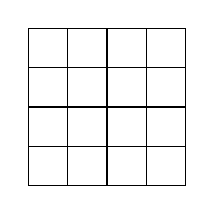
\begin{tikzpicture}[every node/.style={font=\small, align=center}]
    \foreach \i in {0,1,2,3} {
        \foreach \j in {0,1,2,3} {
            \draw[thin] (\i*0.5, \j*0.5) rectangle (\i*0.5+0.5, \j*0.5+0.5);
        }
    }
\end{tikzpicture}
\caption{MAE step 1: original image. The image is divided into a $4 \times 4$ grid of non-overlapping patches. Real MAE uses $14 \times 14$ patches on $224 \times 224$ inputs; the small grid here is a schematic.}
\label{fig:mae_original}
\end{figure}

\begin{figure}
\centering
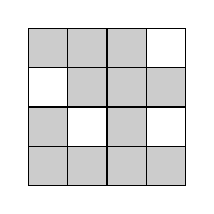
\begin{tikzpicture}[every node/.style={font=\small, align=center}]
    \foreach \mi/\mj in {0/0, 0/1, 0/3, 1/0, 1/2, 1/3, 2/0, 2/1, 2/2, 2/3, 3/0, 3/2} {
        \fill[black!20] (\mi*0.5, \mj*0.5) rectangle (\mi*0.5+0.5, \mj*0.5+0.5);
    }
    \foreach \i in {0,1,2,3} {
        \foreach \j in {0,1,2,3} {
            \draw[thin] (\i*0.5, \j*0.5) rectangle (\i*0.5+0.5, \j*0.5+0.5);
        }
    }
\end{tikzpicture}
\caption{MAE step 2: $75\%$ of patches masked. Twelve of the sixteen patches are replaced with mask tokens (filled grey); only the four visible patches reach the encoder. The high mask ratio forces the encoder to integrate global structure rather than relying on local interpolation from neighbouring patches.}
\label{fig:mae_masked}
\end{figure}

\begin{figure}
\centering
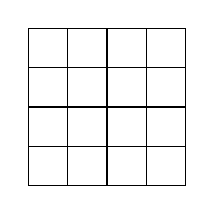
\begin{tikzpicture}[every node/.style={font=\small, align=center}]
    \foreach \i in {0,1,2,3} {
        \foreach \j in {0,1,2,3} {
            \draw[thin] (\i*0.5, \j*0.5) rectangle (\i*0.5+0.5, \j*0.5+0.5);
        }
    }
\end{tikzpicture}
\caption{MAE step 3: reconstruction. The encoder produces representations of the visible patches, and a lightweight decoder reconstructs all sixteen patches including the masked ones. The decoder is small and is discarded after pre-training; the encoder is the part that transfers to downstream tasks.}
\label{fig:mae_reconstructed}
\end{figure}

\vspace{1.5em}

\newthought{Knowledge Distillation.}\index{knowledge distillation}\cite{HintonDistillation2015}
Knowledge distillation is not a self-supervised method on its own, but it is the bridge that connects masked prediction in pixel space to masked prediction in feature space.
The original idea is to compress a large teacher into a smaller student by training the student to match the teacher's soft output distribution rather than hard labels.
The soft labels are produced by scaling the teacher's logits with a temperature $T$:

\begin{align*}
    p_i^{(T)} &= \frac{\exp(z_i / T)}{\sum_j \exp(z_j / T)}
\end{align*}

Higher $T$ yields a softer distribution that reveals the structure of the teacher's uncertainty across classes.
The student inherits not just the teacher's predictions but the geometry of its decision boundary, which carries far more information per example than a one-hot label would.

\vspace{1.5em}

\newthought{Data2Vec.}\index{Data2Vec}\cite{Baevski2022Data2Vec}
Data2Vec generalises masked prediction across modalities by predicting in feature space rather than input space.
A teacher network produces target representations from the unmasked input, and a student network predicts those representations from a masked version of the same input.
The same recipe applies to vision, speech, and text; the only thing that changes is the modality-specific tokeniser.
Predicting latent representations sidesteps the awkward question of what the right reconstruction loss is for each modality, since the target lives in a learned space rather than in raw pixels, audio samples, or token indices.

\newthought{Masking still confines supervision to a single modality.}
Each modality's pretext task respects its own boundaries: BERT masks tokens, MAE masks patches, Data2Vec masks features within one modality at a time.
What if two modalities together supplied a stronger signal, with each modality acting as the supervision for the other?


\subsection{Cross-Modal Self-Supervision}\index{CLIP}

\marginnote{\newthought{CLIP.} Contrastive Language-Image Pre-training\cite{Radford2021CLIP} learns from image-caption pairs scraped from the web. The pairing is the supervision; nobody had to label the images with class names.}

\newthought{Cross-modal self-supervision} extends the contrastive idea across modalities.
CLIP trains an image encoder and a text encoder jointly on four hundred million image-caption pairs collected from the web.
For each minibatch, the contrastive task is to match each image to its corresponding caption among all captions in the batch, and each caption to its corresponding image.
The pairing itself is the supervision; nobody had to label the images with class names because the captions came along with them.

\newthought{The result} is a representation in which images and text inhabit the same vector space.
A familiar image embedding sits near the embedding of any reasonable caption that describes it; a familiar caption embedding sits near the embedding of any image it could plausibly describe.
Cosine similarity in this joint space is interpretable as semantic relatedness across modalities.

\begin{figure}
\centering
\begin{tikzpicture}
    \begin{axis}[
        xlabel={$z^{(1)}$}, ylabel={$z^{(2)}$},
        xmin=-3, xmax=3, ymin=-3, ymax=3,
        width=0.5\textwidth, height=0.5\textwidth,
        axis line style={draw=none},
        tick style={black, thin},
        xtick={-2,0,2}, ytick={-2,0,2},
        xticklabel style={font=\small},
        yticklabel style={font=\small},
        tick align=outside, tick pos=left,
    ]
    \addplot[only marks, mark=*, mark size=2pt, black] coordinates {
        (-1.5,1.2) (1.4,0.5) (-0.3,-1.6)
    };
    \addplot[only marks, mark=o, mark size=2pt, black, thick] coordinates {
        (-1.4,1.4) (1.6,0.6) (-0.5,-1.5)
    };
    \draw[densely dashed, black!60] (axis cs:-1.5,1.2) -- (axis cs:-1.4,1.4);
    \draw[densely dashed, black!60] (axis cs:1.4,0.5) -- (axis cs:1.6,0.6);
    \draw[densely dashed, black!60] (axis cs:-0.3,-1.6) -- (axis cs:-0.5,-1.5);
    \node[font=\small, anchor=north east] at (axis cs:-1.5,1.2) {img$_1$};
    \node[font=\small, anchor=south west] at (axis cs:-1.4,1.4) {``a banana''};
    \node[font=\small, anchor=south west] at (axis cs:1.6,0.6) {``a car''};
    \node[font=\small, anchor=south west] at (axis cs:-0.5,-1.5) {``a tree''};
    \end{axis}
\end{tikzpicture}
\caption{CLIP joint embedding space. Filled markers are image embeddings, open markers are text embeddings. The contrastive objective pulls each image toward its corresponding caption (dashed pairings) and pushes it away from all other captions in the batch. After training, an image and a caption that describe the same content land close together in the same vector space.}
\label{fig:clip_joint}
\end{figure}

\newthought{Zero-shot classification} is the immediate consequence.
A new image can be classified without any task-specific training: encode the candidate class names as text prompts (``a photo of a banana'', ``a photo of an apple'', ``a photo of an orange''), encode the image, and pick the class whose text embedding has the highest cosine similarity to the image embedding.
The model has never seen the class label as a training signal, yet it can recognise the class because it has seen many images that were captioned with related words.

\newthought{Trace one zero-shot prediction} through the pipeline to make this concrete.
An image of a banana arrives.
The image encoder produces an embedding $e_I$.
The text encoder produces three candidate embeddings $e_T^{\text{(banana)}}, e_T^{\text{(apple)}}, e_T^{\text{(car)}}$ for the three candidate prompts.
Cosine similarity is computed between $e_I$ and each candidate; the prediction is the class whose text embedding has the highest similarity.
No retraining, no labels, no adaptation step.

\newthought{The use payoff} of cross-modal pre-training is concrete.
A model trained on captions, with no class labels, classifies images of categories it was never explicitly trained on.
The same contrastive principle that pulled augmented views together in SimCLR returns here, but across modalities; image and text become two views of the same underlying concept, and the contrastive loss aligns them.
Self-supervised learning has stopped being a method for cheap pre-training and has become a recipe for representations rich enough to handle tasks they were never explicitly trained for.

\newthought{The encoder is now strong enough to teach.}
Once the contrastive, non-contrastive, and masked-prediction recipes give us a representation that captures semantic structure, a question opens up that did not exist when the encoder was random.
What if a small labelled set on the downstream task was paired with a much larger unlabelled set drawn from the same distribution, and the encoder's own predictions were used as supervision on the unlabelled portion?
That is the semi-supervised regime, and the methods in the next two subsections turn the SSL flywheel one more turn: representations from raw data, then pseudo-labels from those representations, then a stronger model from the pseudo-labels.


\subsection{Pseudo-Labels and Self-Training}\index{pseudo-labelling}\index{self-training}

\marginnote{\newthought{Pseudo-labelling.} The model writes the labels it then learns from\cite{Lee2013PseudoLabel}. The signal comes from the model's own confidence, not from a human.}

\newthought{Pseudo-labelling} is the simplest way to use unlabelled data once the encoder is good enough to be trusted on parts of it.
Train a classifier on the small labelled set $\mathcal{L}$, run it on the unlabelled set $\mathcal{U}$, keep the predictions whose confidence exceeds a threshold $\tau$, and add those high-confidence predictions to $\mathcal{L}$ as if they were ground truth.
Retrain on the expanded labelled set, predict again, and repeat.
The encoder learned the geometry from raw data; the classifier learns the labels from itself.

\vspace{1.5em}

\begin{algorithm}[H]
\caption{Pseudo-Labelling with Confidence Thresholding}
\begin{algorithmic}[1]
\Require Labelled set $\mathcal{L}$, unlabelled set $\mathcal{U}$, threshold $\tau$
\State Train classifier $f$ on $\mathcal{L}$
\Repeat
    \For{each $x \in \mathcal{U}$}
        \State $\hat{p} \gets f(x)$, $\hat{y} \gets \arg\max \hat{p}$
        \If{$\max(\hat{p}) > \tau$}
            \State Add $(x, \hat{y})$ to $\mathcal{L}$
            \State Remove $x$ from $\mathcal{U}$
        \EndIf
    \EndFor
    \State Retrain $f$ on the expanded $\mathcal{L}$
\Until{convergence or $\mathcal{U}$ is empty}
\end{algorithmic}
\end{algorithm}

\newthought{Notice that the threshold $\tau$ is the only design choice that matters.}
A high $\tau$ keeps the pseudo-label set small but accurate; a low $\tau$ adds many examples but admits more errors.
A common protocol is curriculum thresholding: start with $\tau$ near $0.95$, lower it gradually as the classifier improves, so the easy points enter the labelled set first and the hard points enter only when the classifier has earned the right to label them.

\newthought{Confirmation bias} is the central failure mode\index{confirmation bias} and the reason pseudo-labelling cannot be run blindly.
The model makes an error on an unlabelled point, that error becomes a pseudo-label, the next round of training treats the wrong label as correct, and the model becomes more confident in the same mistake.
The loop is self-reinforcing in exactly the wrong direction; the very confidence that gates the pseudo-label is the property the loop inflates.

\newthought{Calibration is the fix} that makes the threshold mean what we think it means.
A neural network is well-calibrated\index{calibration} when $P(\hat{y} = y \mid \hat{p} = p) = p$, that is, when an event the network claims with probability $0.9$ actually happens nine times out of ten.
Modern networks are systematically overconfident, especially on out-of-distribution inputs and near decision boundaries\cite{Guo2017Calibration}.
Temperature scaling adjusts logits before the softmax,

\begin{align*}
    \hat{p}_{\text{calibrated}} &= \mathrm{softmax}(z / T)
\end{align*}

with a single scalar $T > 1$ fitted on a held-out validation set; the rank of predictions is preserved, but the confidences are stretched toward truthful values.
A calibrated $\tau{=}0.95$ keeps roughly five percent error in the pseudo-label set; an uncalibrated $\tau{=}0.95$ keeps whatever error the network's overconfidence happens to produce.

\marginnote{\newthought{Calibration before pseudo-labelling.} Always temperature-scale the classifier on a held-out set before reading off confidences as a threshold. Otherwise the threshold gates on a signal that the network has been trained to inflate.}


\subsection{Consistency Regularisation and FixMatch}\index{consistency regularisation}\index{FixMatch}

\marginnote{\newthought{Consistency.} Predictions should be stable under perturbations that preserve the class. The unlabelled point gets a target derived from itself.}

\newthought{Consistency regularisation} attacks the same problem from the loss side.
The pseudo-label algorithm uses confident predictions as hard targets; consistency uses the prediction itself as the target on a perturbed view of the same input.
The intuition is the same one that drove SimCLR's positive pairs: if a small augmentation changes the input but not the class, the model's prediction should not change either.

\begin{align*}
    \mathcal{L}_{\text{consistency}} &= \sum_{x \in \mathcal{U}} d\bigl(f(x),\, f(\mathrm{aug}(x))\bigr)
\end{align*}

where $\mathrm{aug}$ is a stochastic augmentation and $d$ is a distance such as mean squared error or KL divergence between predicted distributions.
No threshold, no confirmation bias loop; the model trains itself to be invariant to augmentation, and the unlabelled set becomes a regulariser rather than a label source.

\newthought{Mean Teacher} stabilises consistency by using a slow-moving copy of the network as the target\cite{Tarvainen2017MeanTeacher}.\index{Mean Teacher}
The student updates by gradient descent; the teacher updates as an exponential moving average of the student weights,

\begin{align*}
    \theta_{\text{teacher}} &\gets \alpha\, \theta_{\text{teacher}} + (1 - \alpha)\, \theta_{\text{student}}
\end{align*}

with $\alpha$ typically near $0.99$.
The student matches the teacher's predictions on the same input under different augmentations; the teacher lags the student so its predictions act as a stable target rather than a moving one.
The mechanism is the same one MoCo used to stabilise its key encoder, transplanted into semi-supervised classification.

\marginnote{\newthought{Why EMA helps.} A teacher that updates as fast as the student tracks the same noise the student does; an averaged teacher smooths over recent fluctuations and presents the student with a target the loss can actually reduce.}

\vspace{1.5em}

\newthought{Co-training} attacks the confirmation bias problem from a different angle: use two classifiers, each trained on a different view of the data, and let each one label data for the other\cite{Blum1998CoTraining}.\index{co-training}
The assumption is that the two views are conditionally independent given the label, so an error one classifier makes on its own view is not an error the other classifier is likely to make on its view.
For web pages the canonical split is page content versus anchor text from incoming links; for sensors it might be one modality versus another, or one half of the feature vector versus the other.
When the conditional independence holds, the two classifiers correct each other; when it does not, they share blind spots and confirmation bias returns through the back door.

\newthought{Tri-training} relaxes the independence assumption by replacing it with agreement\index{tri-training}.
Train three classifiers on bootstrapped subsets of the labelled data, and pseudo-label an unlabelled point for the third classifier only when the other two agree on it.
The disagreement signal does the filtering that conditional independence was supposed to do; if two independently bootstrapped classifiers both produce the same prediction, that prediction is more likely to be right than either one alone.

\vspace{1.5em}

\newthought{FixMatch} is the synthesis of all of the above\cite{Sohn2020FixMatch}.\index{FixMatch}
Take an unlabelled image, apply a weak augmentation such as flip and crop, and read the model's prediction; if the confidence exceeds $\tau$, accept the prediction as a pseudo-label.
Then apply a strong augmentation such as RandAugment to the same image, and train the model to match the pseudo-label on the strongly augmented view.
Weak augmentation produces a trustworthy target; strong augmentation produces a hard training signal; the loss couples the two.

\begin{align*}
    \mathcal{L}_{\text{FixMatch}} &= \mathcal{L}_{\text{supervised}} + \lambda \sum_{x \in \mathcal{U}} \mathbf{1}\!\bigl[\max \hat{p}_w > \tau\bigr]\, H\bigl(\hat{y}_w,\, f(x_{\text{strong}})\bigr)
\end{align*}

where $\hat{p}_w$ is the prediction on the weakly augmented view, $\hat{y}_w$ is its argmax, $x_{\text{strong}}$ is the strongly augmented view, $H$ is cross-entropy, and $\lambda$ balances supervised and unsupervised terms.

\begin{algorithm}[H]
\caption{FixMatch}
\begin{algorithmic}[1]
\Require Labelled batch $\mathcal{B}_L$, unlabelled batch $\mathcal{B}_U$, threshold $\tau$, weight $\lambda$
\State Compute supervised loss $\mathcal{L}_s$ on $\mathcal{B}_L$
\For{each $x \in \mathcal{B}_U$}
    \State $x_w \gets \mathrm{weak}(x)$, $\hat{p}_w \gets f(x_w)$, $\hat{y}_w \gets \arg\max \hat{p}_w$
    \If{$\max \hat{p}_w > \tau$}
        \State $x_s \gets \mathrm{strong}(x)$
        \State Accumulate $H(\hat{y}_w, f(x_s))$ into the unsupervised loss $\mathcal{L}_u$
    \EndIf
\EndFor
\State Update $\theta$ by gradient descent on $\mathcal{L}_s + \lambda \mathcal{L}_u$
\end{algorithmic}
\end{algorithm}

\newthought{Notice that FixMatch makes the asymmetry between weak and strong explicit.}
The weak view exists to extract a label the model already trusts; the strong view exists to make the model robust against perturbations it does not yet handle.
Reverse the assignment, ask for pseudo-labels from strongly augmented views, and the labels are too noisy to be useful; train on weakly augmented views, and the model learns nothing it did not already know.
The two augmentation regimes have different jobs.

\begin{figure}
\centering
\begin{tikzpicture}[
    every node/.style={font=\small, align=center},
    block/.style={rectangle, draw=black, thick, rounded corners=2pt,
                  minimum width=1.6cm, minimum height=0.7cm, inner sep=4pt},
    arr/.style={-{Triangle[length=4pt, width=4pt, fill=black!70]}, thick, black!70},
]
    \node[block] (x) at (0,0) {unlab.\ $x$};
    \node[block] (weak) at (2.6, 1.2) {weak aug};
    \node[block] (strong) at (2.6,-1.2) {strong aug};
    \node[block, fill=black!8] (m1) at (5.0, 1.2) {$f$};
    \node[block, fill=black!8] (m2) at (5.0,-1.2) {$f$};
    \node[block] (gate) at (7.4, 1.2) {$\max\hat{p}_w {>} \tau$?};
    \node[block] (pl) at (7.4, 0) {$\hat{y}_w$};
    \node[font=\small] (loss) at (9.4,-1.2) {$H(\hat{y}_w, f(x_s))$};

    \draw[arr] (x) -- (weak);
    \draw[arr] (x) -- (strong);
    \draw[arr] (weak) -- (m1);
    \draw[arr] (strong) -- (m2);
    \draw[arr] (m1) -- (gate);
    \draw[arr] (gate) -- node[right, font=\tiny] {yes} (pl);
    \draw[arr] (pl) -| (loss.north);
    \draw[arr] (m2) -- (loss.west);
\end{tikzpicture}
\caption{FixMatch. The same unlabelled $x$ produces a weakly augmented view that gates a pseudo-label and a strongly augmented view that receives the cross-entropy loss. The pseudo-label only fires when the weak-view confidence exceeds the threshold $\tau$, so the unsupervised loss is silent on uncertain examples.}
\label{fig:fixmatch}
\end{figure}

\newthought{Model-in-the-loop labelling} closes the loop back to the foundation models from earlier in this chapter and to chapter 8's CLIP and SAM.
A large pre-trained model proposes labels on unlabelled data; a human reviews and corrects them; the corrected labels train the smaller downstream model.
Verifying a candidate label is much faster than producing one from scratch, and the foundation model's representations are good enough that its proposals are right most of the time.
GPT-style models can propose named-entity annotations for review, SAM can propose segmentation masks for correction, and CLIP can propose image classifications that a human triages.
The pattern is the same one the rest of this chapter built up to: the encoder learned from raw data is now strong enough to do most of the labelling work itself, and the human supplies the part the encoder cannot.


% ==============================================================================================
% BLOCK 3: STUDENT ACTIVATION
% ==============================================================================================

\newpage

\section{Examples \& Exercises}\index{examples}\index{exercises}

\marginnote{\newthought{Exercises} are for practice and reinforcing concepts. Try to solve them on your own first,
try things, play with it, discuss, this is not a time trial. And there is no shame in not ending up at the right answer,
in the same sense, that uncovering great questions
and tossing them around is usually pretty fruitful on the long run.}

\newthought{Computing by hand} builds the intuition that no SimCLR batch can replace.
Step through the arithmetic slowly.

\vspace{1em}

\newthought{Design a pretext task.}
Propose a self-supervised pretext task for each of the following modalities, specifying the input transformation, the prediction target, and the structural property of the data that makes the supervision free.

\begin{itemize}
    \item Audio data, for example raw speech recordings.
    \item Time series, for example multivariate sensor readings from a manufacturing line.
    \item Graphs, for example molecular structures with node and edge attributes.
\end{itemize}

\marginnote{\newthought{Sketch.} Audio: predict the next short audio chunk from past chunks (autoregressive), or contrast two augmented views of the same clip against clips from other recordings (contrastive). Time series: mask out a window of values and predict it from the surrounding context, mirroring BERT. Graphs: mask edges or node features and predict them from the rest of the graph, or contrast two perturbed views of the same graph against views of others. The structural property in each case is locality: nearby slices in time, nearby tokens in text, nearby nodes in a graph share more information than distant ones.}

\vspace{2.5em}

\newthought{InfoNCE loss by hand.}
You have an anchor representation $z$ with one positive and two negatives, with cosine similarities $\mathrm{sim}(z, z^+) = 0.9$, $\mathrm{sim}(z, z^-_1) = 0.3$, and $\mathrm{sim}(z, z^-_2) = 0.1$.
Compute $\mathcal{L}_{\text{InfoNCE}}$ from Equation~\ref{eq:infonce} with temperature $\tau = 0.5$.

\newthought{Numerator.}
\begin{align*}
    \exp(0.9 / 0.5) &= \exp(1.8) \\
                    &\approx 6.05
\end{align*}

\newthought{Denominator.}
\begin{align*}
    \sum &= \exp(1.8) + \exp(0.6) + \exp(0.2) \\
         &\approx 6.05 + 1.82 + 1.22 \\
         &\approx 9.09
\end{align*}

\newthought{Loss.}
\begin{align*}
    \mathcal{L}_{\text{InfoNCE}} &= -\log\!\left(\tfrac{6.05}{9.09}\right) \\
                                  &\approx -\log(0.665) \\
                                  &\approx 0.41
\end{align*}

The positive dominates the denominator, so the loss is small but not zero.
Bring the negatives closer in similarity, or lower the temperature, and the loss climbs sharply.

\marginnote{\newthought{Temperature shapes the gradient.} Halving $\tau$ to $0.25$ turns the same similarities into $\exp(3.6), \exp(1.2), \exp(0.4)$, and the positive's share of the denominator jumps from $0.67$ to $0.92$. The loss falls because the easy positive looks even easier; a harder positive would have produced the opposite move. Doubling $\tau$ to $1.0$ flattens the softmax: the positive's share is $0.46$, the loss climbs to $0.78$, and the gradient is shared more evenly across all candidates.}

\vspace{2.5em}

\newthought{InfoNCE on the canonical six points.}
Take $x_1 = (1,2)$ and $x_4 = (6,8)$ as the two anchors.
Generate small augmentations by adding noise: $x_1' = (1.2, 2.3)$ and $x_4' = (5.8, 8.1)$.
The positive pair for $x_1$ is $(x_1, x_1')$; the negatives are $x_4$ and $x_4'$.
Compute cosine similarity between $x_1$ and each of the other three vectors, then write down the InfoNCE loss for the positive pair $(x_1, x_1')$ at temperature $\tau = 0.1$.

The cosine similarity between $x_1$ and $x_1'$ is:

\begin{align*}
    \mathrm{sim}(x_1, x_1') &= \frac{x_1 \cdot x_1'}{\|x_1\|\,\|x_1'\|} \\
                             &= \frac{1 \cdot 1.2 + 2 \cdot 2.3}{\sqrt{5}\,\sqrt{6.73}} \\
                             &= \frac{5.8}{\sqrt{33.65}} \\
                             &\approx \frac{5.8}{5.80} \\
                             &\approx 1.00
\end{align*}

Compute the other two similarities yourself, then verify against the table.

\begin{table*}[ht]
\centering
\begin{tabular}{p{0.18\textwidth}p{0.18\textwidth}p{0.20\textwidth}}
    \toprule
    \textbf{Pair} & \textbf{Cosine sim} & \textbf{$\exp(\cdot/0.1)$} \\
    \midrule
    $(x_1, x_1')$ positive & $\approx 1.00$ & $\approx 22026$ \\
    $(x_1, x_4)$ negative  & $\approx 0.97$ & $\approx 16318$ \\
    $(x_1, x_4')$ negative & $\approx 0.97$ & $\approx 16318$ \\
    \bottomrule
\end{tabular}
\vspace{2em}
\caption{Cosine similarities between $x_1$ and the other three vectors, plus their exponentials at temperature $\tau{=}0.1$. The four points are nearly collinear from the origin, so all three similarities are close to one; the contrastive signal is weak, and the InfoNCE loss is large.}
\label{tab:infonce_six_points}
\end{table*}

\newthought{Loss.}
\begin{align*}
    \mathcal{L}_{\text{InfoNCE}} &= -\log\!\left(\tfrac{22026}{22026 + 16318 + 16318}\right) \\
                                  &\approx -\log(0.40) \\
                                  &\approx 0.92
\end{align*}

\marginnote{\newthought{Why the loss is so large.} The four vectors all sit in roughly the same direction from the origin, so cosine similarity is unable to separate them well. Cosine similarity ignores magnitude, so points along similar rays look almost identical. Pre-processing such as centering or normalising can fix this; in real SimCLR, the projection head transforms representations into a space where directions are meaningful for contrastive learning.}

\vspace{2.5em}

\newthought{Augmentation ablation.}
Why is random cropping the single most important augmentation in SimCLR?
What information does it remove that the network would otherwise rely on, and what would happen to the learned representation if you removed cropping while keeping colour jitter and Gaussian blur?
What augmentations would be appropriate for medical imaging, and which would be inappropriate?

\marginnote{\newthought{Sketch.} Without cropping, two views of the same image differ only in colour and blur, and the network can match them on low-level statistics: average colour, brightness, texture. Cropping forces the views to overlap on different parts of the same object, so matching them requires recognising the object across spatial location. Remove cropping and the representation captures appearance rather than semantics, and downstream classification accuracy drops sharply. For medical imaging, intensity normalisation and small rotations are appropriate; colour jitter is inappropriate because colour often encodes diagnostic information; aggressive cropping is inappropriate because anatomical context matters.}

\vspace{2.5em}

\newthought{Why doesn't collapse happen.}
SimSiam has no negatives, no momentum encoder, no contrastive term, and yet the loss does not collapse to a constant in practice.
Predict the effect of removing each ingredient in turn: the predictor head, the stop-gradient, BatchNorm in the projector.
Rank the three by how quickly removing them causes collapse, and justify your ranking.

\marginnote{\newthought{Sketch.} Removing the predictor head turns the two branches symmetric; collapse is rapid because the trivial constant solution becomes the symmetric fixed point of the loss. Removing the stop-gradient lets both branches update by the same gradient toward the same constant; collapse is rapid here too. Replacing BatchNorm with LayerNorm in the projector weakens the implicit contrastive signal that BatchNorm supplies through batch-level normalisation; collapse is slower but reliable. Ranking by speed of collapse: stop-gradient $\approx$ predictor (both load-bearing) $\gtrsim$ BatchNorm. The redundancy is part of why SimSiam is robust; the dependence is part of why it is fragile.}

\vspace{2.5em}

\newthought{Masked language modelling loss.}
Consider a five-token sentence ``the cat sat on mat'' where positions $2$ (``cat'') and $5$ (``mat'') are masked.
The model produces predicted distributions over the vocabulary at each masked position; the entries on the original tokens are $p(\text{cat}) = 0.7$ and $p(\text{mat}) = 0.4$.
Compute the MLM loss from Equation~\ref{eq:mlm}.

\begin{align*}
    \mathcal{L}_{\text{MLM}} &= -\bigl(\log 0.7 + \log 0.4\bigr) \\
                              &\approx -(-0.357 + (-0.916)) \\
                              &\approx 1.27
\end{align*}

\marginnote{\newthought{What the number means.} The loss is the sum of negative log probabilities at masked positions, averaged over the masked count; per masked token, the average loss here is $0.64$. A perfectly confident model on the right tokens would have loss $0$. Cross-entropy of $0.64$ corresponds to the model assigning roughly $\exp(-0.64) \approx 0.53$ probability to the right token on average, which is a learning model but not a finished one.}

\vspace{2.5em}

\newthought{MoCo queue dynamics.}
A MoCo training run starts with an empty queue of size $K = 8$ and processes minibatches of size $4$.
After three minibatches, what does the queue contain, and what does the momentum encoder weight look like under update rule $\theta_k \gets m\,\theta_k + (1-m)\,\theta_q$ with $m = 0.99$?

After minibatch $1$: queue has 4 entries (the 4 keys from this batch), momentum encoder weights are $\theta_k^{(1)} = 0.99\,\theta_k^{(0)} + 0.01\,\theta_q^{(1)}$.

After minibatch $2$: queue has 8 entries (full), momentum encoder weights drift further toward $\theta_q^{(2)}$.

After minibatch $3$: the oldest 4 keys are evicted to make room for the new 4; queue still has 8 entries, and the momentum encoder weights have absorbed about $3\%$ of the current online encoder.

\marginnote{\newthought{Why $m{=}0.99$ matters.} A momentum of $0.99$ means each minibatch contributes only $1\%$ of the change; after one hundred minibatches, the key encoder has lagged the online encoder by roughly $100 \cdot 0.01 = 1$ full update worth. With $m{=}0.999$ the lag is ten times longer; with $m{=}0.9$ the queue would be inconsistent on the timescale of a few updates, defeating the point. The momentum is the parameter that buys consistency; it is the load-bearing knob in MoCo.}

\vspace{2.5em}

\newthought{CLIP zero-shot inference.}
Given an image embedding $e_I = (0.7, 0.6, 0.4)$ and three candidate text embeddings:

\begin{itemize}
    \item $e_T^{\text{(banana)}} = (0.8, 0.5, 0.3)$
    \item $e_T^{\text{(apple)}} = (0.2, 0.9, 0.4)$
    \item $e_T^{\text{(car)}} = (-0.4, 0.1, 0.8)$
\end{itemize}

Compute the cosine similarity between the image and each candidate, then pick the predicted class.

For the banana candidate:

\begin{align*}
    e_I \cdot e_T^{\text{(banana)}} &= 0.7 \cdot 0.8 + 0.6 \cdot 0.5 + 0.4 \cdot 0.3 \\
                                     &= 0.56 + 0.30 + 0.12 \\
                                     &= 0.98 \\[4pt]
    \|e_I\| &= \sqrt{0.49 + 0.36 + 0.16} \\
            &= \sqrt{1.01} \\
            &\approx 1.005 \\[4pt]
    \|e_T^{\text{(banana)}}\| &= \sqrt{0.64 + 0.25 + 0.09} \\
                              &= \sqrt{0.98} \\
                              &\approx 0.990 \\[4pt]
    \mathrm{sim} &= \frac{0.98}{1.005 \cdot 0.990} \\
                 &\approx 0.985
\end{align*}

Compute the other two similarities and verify against the table:

\begin{table*}[ht]
\centering
\begin{tabular}{p{0.16\textwidth}p{0.16\textwidth}p{0.16\textwidth}p{0.16\textwidth}}
    \toprule
    \textbf{Class} & \textbf{$e_I \cdot e_T$} & \textbf{$\|e_T\|$} & \textbf{Cosine sim} \\
    \midrule
    banana & $0.98$ & $0.990$ & $0.985$ \\
    apple  & $0.84$ & $1.005$ & $0.832$ \\
    car    & $0.06$ & $0.900$ & $0.066$ \\
    \bottomrule
\end{tabular}
\vspace{2em}
\caption{CLIP zero-shot scoring. The image embedding has highest cosine similarity to the banana text embedding; the prediction is banana, with no model retraining and no labelled banana examples.}
\label{tab:clip_zero_shot}
\end{table*}

\marginnote{\newthought{What temperature would change.} Real CLIP applies a temperature to the similarities before taking the softmax across class candidates: $\mathrm{softmax}(\mathrm{sim}/\tau)$. A small $\tau$ sharpens the prediction toward the top class; a large $\tau$ produces a more diffuse class probability distribution that is useful when downstream code wants soft outputs rather than hard predictions.}

\vspace{2.5em}

\newthought{Pseudo-labelling threshold.}
You have $100$ unlabelled points and a classifier whose predictions and ground truth break down as follows: $20$ points have confidence above $0.95$, of which $18$ are correct; $30$ points have confidence between $0.80$ and $0.95$, of which $21$ are correct; $50$ points have confidence below $0.80$, of which $25$ are correct.
Compute the pseudo-label accuracy at $\tau = 0.95$ and at $\tau = 0.80$, and decide which threshold you would deploy.

\vspace{0.5em}

At $\tau = 0.95$ the pseudo-label set has $20$ entries and $18$ are correct, for an accuracy of $0.90$.
At $\tau = 0.80$ the pseudo-label set has $50$ entries and $39$ are correct, for an accuracy of $0.78$.

\marginnote{\newthought{Which threshold.} The high threshold trades coverage for accuracy. With $\tau{=}0.95$ you add $20$ clean pseudo-labels per round; with $\tau{=}0.80$ you add $50$ but with eleven extra wrong labels. The right answer depends on how robust the next round of training is to label noise; for a small classifier with limited capacity, the cleaner set wins, and curriculum thresholding lets you start at $0.95$ and lower toward $0.80$ once the classifier has stabilised.}

\vspace{2.5em}

\newthought{Confirmation bias by example.}
A sentiment classifier trained on a small labelled set repeatedly misclassifies ironic positive reviews as negative, because the labelled set contains few examples of irony.
Trace through what happens over three rounds of self-training: which pseudo-labels enter the training set, what the classifier does on the next round, and what the loss looks like as the training set grows.
What property of the labelled set caused the failure, and what would calibrating the classifier before pseudo-labelling change?

\marginnote{\newthought{Sketch.} Round one: confident negative predictions on ironic positives enter the pseudo-label set as wrong negatives. Round two: the training set now contains more wrong-negative ironic examples, so the classifier becomes more confident that irony is negative; the loss falls because the classifier matches its own wrong labels. Round three: the bias is cemented; novel ironic positives are pseudo-labelled as negative with even higher confidence. The root cause is that the labelled set was unrepresentative of the input distribution; calibrating helps only if it pulls the wrong predictions below the threshold, which is unlikely once overconfidence has set in. The real fix is data: a small set of labelled ironic examples breaks the loop.}

\vspace{2.5em}

\newthought{FixMatch design choice.}
FixMatch reads a pseudo-label off the weakly augmented view and trains the classifier to match it on the strongly augmented view.
Why this asymmetry?
Predict what would happen if both views used weak augmentation, and what would happen if both used strong augmentation.
Which of the two failure modes does FixMatch's actual design avoid, and why is the other one less of a concern?

\marginnote{\newthought{Sketch.} Both weak: pseudo-labels are trustworthy but the model never sees a hard training signal, so it learns nothing the supervised loss did not already teach. Both strong: pseudo-labels are noisy because strong augmentation perturbs the prediction, and the model trains on its own noise. FixMatch's actual design avoids the second failure, the more dangerous one, because noisy pseudo-labels feed confirmation bias directly. The first failure is benign in comparison: the model is conservative but not actively wrong. The asymmetry lets FixMatch get the trustworthy target from the easy view and the hard training signal from the difficult view.}

\vspace{2.5em}

% ============================= CODE ===============================

\marginnote{\newthought{Code} will be provided as a Python notebook.
Use it as a starting point, break things, and observe what changes.}
\marginnote{CIFAR-10 subset, 5\,000 images\\ten classes, 32$\times$32 pixels\\[4pt]implement: SimCLR augmentation pipeline, InfoNCE loss, linear evaluation protocol}

\newthought{A vision dataset to explore.}
You are given 5\,000 CIFAR-10 images without labels.
Implement the SimCLR augmentation pipeline of random crop, colour jitter, and Gaussian blur.
Train a small two-layer MLP encoder with the InfoNCE loss.
Evaluate the learned representations by fitting a linear classifier on top of the frozen encoder, and compare the linear-evaluation accuracy of your SSL-pretrained encoder against an encoder trained from scratch on only 100 labelled examples.

\newthought{What to observe.}
SSL pre-training on unlabelled data consistently outperforms a randomly initialised encoder trained on very few labels; the pre-trained features are general enough that a linear head can pick up the class structure with limited supervision.
The quality of the learned representation depends heavily on the augmentation pipeline; weak augmentations (small crops, mild colour jitter) yield shortcut features that do not transfer, and the linear evaluation accuracy gap collapses.
Temperature $\tau$ controls the sharpness of the contrastive distribution; too low and the loss collapses onto the hardest negatives, producing a representation that distinguishes only the closest competitors; too high and the model treats every negative the same and ignores fine-grained similarity, producing an undifferentiated representation.
The trade-off is the same one you saw in the InfoNCE-by-hand exercise, played out at scale.


\section{Self-Reflection and Recap}\index{reflection}\index{recap}

\newthought{Self-Reflection} questions to guide your thinking:
\begin{itemize}
    \item What failure modes arise when a pretext task is too easy, and what shortcuts might the network exploit instead of learning useful representations?
    \item How does the temperature $\tau$ in InfoNCE shape the gradient, and what is the trade-off between low and high values?
    \item Why is the projection head discarded after training in SimCLR, and what kind of information does it absorb that we do not want in the downstream representation?
    \item What is the queue size in MoCo a trade-off between, and why does the momentum encoder need to lag the online encoder?
    \item What prevents collapse in non-contrastive methods like BYOL and SimSiam, and which structural ingredient is most load-bearing?
    \item Why is BERT's masking ratio fifteen percent while MAE's is seventy-five percent, and what property of the input distinguishes the two regimes?
    \item Why does cross-modal pre-training as in CLIP enable zero-shot transfer to classes the model never explicitly trained on?
    \item How does FixMatch's split between weak augmentation for pseudo-labels and strong augmentation for training mitigate confirmation bias compared to plain pseudo-labelling, and what would break if the two augmentation regimes were swapped?
    \item Why does pseudo-labelling depend on calibration, and how does the temperature scaling fix relate to the threshold $\tau$ in the algorithm?
    \item When does the conditional independence assumption in co-training hold, and how does tri-training relax it without giving up on the multi-view idea?
\end{itemize}

\newthought{Recap} of Key Concepts:
\begin{itemize}
    \item Self-supervised learning derives free supervision from data structure; the pretext task is scaffolding, the learned representation is the product, and the choice of pretext determines what invariances the representation acquires.
    \item Contrastive methods pull positive pairs together and push negatives apart through the InfoNCE loss; SimCLR realises this with strong augmentations and large batches, and MoCo decouples the negative pool from the batch with a queue and momentum encoder.
    \item Non-contrastive methods such as BYOL and SimSiam avoid collapse through asymmetry, stop-gradient, and BatchNorm, eliminating the need for negative examples; the trivial constant solution is always a fixed point of the loss, and architecture, not loss, prevents convergence to it.
    \item Masked prediction reconstructs hidden inputs from visible context; BERT applies this to language at fifteen percent masking, MAE to vision at seventy-five percent masking, and Data2Vec to any modality in feature space.
    \item Cross-modal pre-training as in CLIP aligns image and text representations through contrastive matching of caption pairs, enabling zero-shot classification at inference without any task-specific training.
    \item Pseudo-labelling expands the labelled set with confident model predictions; confirmation bias is its central failure mode, and calibrating the classifier with temperature scaling is what makes the threshold $\tau$ mean what we want it to mean.
    \item Consistency regularisation forces predictions to be stable under augmentation, with Mean Teacher providing a slow EMA target so the student chases a stable signal rather than its own noise.
    \item FixMatch synthesises pseudo-labelling and consistency: a weakly augmented view supplies a trustworthy pseudo-label, and a strongly augmented view receives the cross-entropy loss against it, with the threshold $\tau$ silencing the unsupervised term on uncertain examples.
\end{itemize}

\marginnote{\newthought{The fundamental dependency.} Every SSL method in this chapter still requires unlabelled data from the target distribution; shift the distribution and the representations degrade, just as the uncertainty methods of chapter 7 degrade under the same drift.}

\newthought{Self-supervised representations are powerful, but they are bound to the distribution they were trained on.}
A SimCLR model pre-trained on natural images will produce useful features for photographs, but it will transfer poorly to medical scans or satellite imagery whose visual statistics differ fundamentally from web data.
The pseudo-labelling and FixMatch loop we just added inherits the same constraint: it leans on the encoder's confidence, and the encoder is only confident where the data resembles what it has already seen.

\newthought{The model writing its own labels is one way to soften the annotation bottleneck; humans writing rough labels is the other.}
Self-training treats the encoder as the source of supervision and lets the human supply only a small clean set; weak supervision goes the other way, asking humans to write noisy heuristics or labelling functions that cover the unlabelled data at scale, and then learning to denoise the resulting overlapping signals.
The two approaches are complements: self-training trusts the model, weak supervision trusts the labelling rules, and both build on the assumption that some signal is better than no signal as long as we know how to handle the noise.

\marginnote{\newthought{Teaser.} If the model can label itself with confidence thresholds, what changes when it is humans who write the noisy labels, and how do we tell apart the cases where a labelling rule is wrong from the cases where it is simply incomplete?}

\newthought{The next chapter explores weak supervision and labelling functions,} where humans contribute heuristics and proxy signals instead of clean annotations, and a label model learns to combine the conflicting outputs into a single training signal.
The flywheel keeps turning: representations from raw data, pseudo-labels from confident representations, and now noisy labels from rough human rules, each loop softening the annotation bottleneck a little further.

\marginnote{\newthought{feedback}}
